\documentclass[10pt]{beamer}

\ifx\pdftexversion\undefined
\usepackage[dvips]{graphicx}
\else
%\usepackage[pdftex]{graphicx}
\DeclareGraphicsRule{*}{mps}{*}{}
\fi

\usepackage[english]{babel}
\usepackage[T1]{fontenc}
\usepackage[utf8]{inputenc}
\usepackage{amsmath}
\usepackage{bbold}
\usepackage[french]{algorithm2e}
\usepackage{multimedia}
\usepackage{tikz}

\definecolor{dark-green}{rgb}{0.2,0.8,0.2}
\useoutertheme{infolines}

\usetheme{Berlin}
\usecolortheme{dolphin}
\beamertemplatenavigationsymbolsempty
\addtobeamertemplate{navigation symbols}{}{%
    \usebeamerfont{footline}%
    \usebeamercolor[fg]{footline}%
    \hspace{1em}%
    \normalsize
    \insertframenumber/\inserttotalframenumber
}

\newcommand{\beginbackup}{
   \newcounter{framenumbervorappendix}
   \setcounter{framenumbervorappendix}{\value{framenumber}}
}
\newcommand{\backupend}{
   \addtocounter{framenumbervorappendix}{-\value{framenumber}}
   \addtocounter{framenumber}{\value{framenumbervorappendix}} 
}

\setbeamercovered{transparent} 

\title{State set representation for hybrid system reachability analysis}
\author[Owen Rouillé]{Owen Rouillé\\[0.3cm]
\footnotesize
Supervised by \textbf{Erika Ábrahám} and \textbf{Stefan Schupp}
}

%\titlegraphic{
%\scalebox{0.4}{
%    		\includegraphics[scale=0.10]{images/LogoENS.eps} \hspace{1.0cm}
%    		\includegraphics[scale=0.6]{images/LogoUnivRennes1.pdf} \hspace{0.5cm}
%        	\includegraphics[scale=0.35]{images/LogoInria.eps} \hspace{0.5cm}
%        	\includegraphics[scale=0.65]{images/LogoHybrid.eps}
%        }
%}

\begin{document}
\maketitle

\section{Introduction}
Computer scientists are used to deal with discrete systems, i.e. systems whose evolution can be described by a sequence of discrete state changes. A widespread example is the program analysis: during the execution of a program, the system is abstracted into a machine which states changes every time an instruction is executed.
Today, computer science is expected to be able to ensure the safety of very complex systems, such as planes or nuclear reactors, which state are described non only by a controller, which is discrete, but also by physical variables, which evolve continuously over the time. Such systems, with a continuous and a discrete component are called hybrid systems. These systems are omnipresent, whenever a computer interacts with continuous quantities there is an hybrid system, even for thing as simple as a thermostat with the temperature.


To study these systems, they are abstracted into hybrid automata. These automata are then model checked. As an example let's take a thermostat, which correspond to an hybrid system, and turn it into an hybrid automata.

An hybrid system is described by a set of possible discrete states and a set of continuous variables. The evolution of the variables is determined by the current discrete state. The current state of the system is defined by the discrete state it is in and by the current value of the continuous variables. A transition between two discrete states can be done under certain conditions (called a guard) over the variables, a well as staying in a given state (called the invariant of the state). A transition can reassign the variables.  

\begin{example} heat controller
\end{example}

\begin{table}
\centering
\begin{tabular}{| c | c | c | c | c |}
	\hline	
	Sub- & derivative & conditions & bounded  & unbounded \\
	classes & & & reachability & reachability \\ \hline
	TA & $\dot x=1$ & $x\overset{?}{=}c$ &\checkmark &\checkmark \\ \hline
	& & $x\overset{?}{\in} [c_1;c_2]$ & &   \\	
   	IRA & $\dot x\in [c_1;c_2]$ & jump must reset &\checkmark &\checkmark \\ 
   	& & $x$ when $\dot x$ changes & &\\ \hline
   	RA & $\dot x\in [c_1;c_2]$ & $x\overset{?}{\in} [c_1;c_2]$ &\checkmark &X \\ \hline
   	LHA I & $\dot x=c$ & $x\overset{?}{=}g_{linear}$ &\checkmark &X \\ \hline
   	LHA II & $\dot x=f_{linear}$ & $x\overset{?}{=}g_{linear}$ &X &X \\ \hline
   	HA  & $\dot x=f$ & $\dot x=g$ &X &X \\ \hline
\end{tabular}
\label{tab_complexity}
\caption{Decidability results for subclasses of automata. $c$, $c_1$, $c_2$ are constants, $f$ and $g$ are function of other variables. TA~=~timed automata, IRA~=~ initialised rectangular automata, RA~=~rectangular automata, LHA I~=~hybrid automata with constant derivatives, LHA~II~=~hybrid automata with linear ODE's, HA~=~general hybrid automata.}
\end{table}

Analyse such systems is very difficult, the table~\ref{tab_complexity} gives the complexity of model checking different classes of automata. Several methods exist to deal with this problem, theorem proving (model for a solver), interval based methods(model it for an SMT solver) and flowpipe computation. This paper contributes to the flowpipe-construction-based reachability analysis methods. The idea is to discretize the time and, at each time step, determine set containing all the possible values for the continuous variables for that time step. The successive representations of the set define a flowpipe=> image.

There exists different sub-methods for the flowpipe construction, each corresponding to different methods to describe the set where of the possible values of the variables. Zonotopes, support functions and boxes are examples of representation. A lot of operations have to performed on these sets along the way, for instance intersections and unions. This paper proposes a method to switch between two representations of polyhedra: the $V$ representation and the $H$ representation according to the theorem~\ref{thm_representation}. First some notations and definitions for the rest of the paper:
 
\begin{definition}[Some geometry]
	The problem is studied in $\mathbb{R}^d$.
	\begin{itemize}
	\item $conv(V)$ defines the convex hull of the set of vertices $V$: $\{ x\in\mathbb{R}^d| x=\sum_{v\in V} \lambda_v v, \sum_{v\in V} \lambda_v =1, \forall v \in V, \ 0\leq \lambda_v \in \mathbb{R} \}$.
	\item $cone(C)$ defines the conic hull of the vectors in $C$: $\{ x\in\mathbb{R}^d| x=\sum_{c\in C} \lambda_c c, \forall c \in C,\ 0\leq \lambda_c \in \mathbb{R} \}$.
	\item $lineal(L)$ is the linear space generated by $L$: $\{ x\in\mathbb{R}^d| x=\sum_{l\in L} \lambda_l l, \forall l \in L,\ \lambda_c \in \mathbb{R} \}$. 
	\item In the paper, a sum between two sets is the Minkowsky sum: $S_1+S_2=\{s_1+s_2|s_1\in S_1,\ s_2 \in S_2 \}$.
	\item An half-space $h$ is an area of $\mathbb{R}^d$ defined by a normal vector $a$ and a constant $b$, $h=\{x\in\mathbb{R}^d|x.a\leq b\}$, its border is the hyperplane $\{x\in\mathbb{R}^d|x.a = b\}$. A family of half-spaces are said independent is their normal vectors are independent, and independent hyperplanes are defined respectively , $d$ independent hyperplanes intersect in a vertex.
	\item Let $A$ be a matrix which rows are normal vectors of a finite set of half-spaces and $B$ the column vector composed by the corresponding constants. $P(A,B)=\{x\in\mathbb{R}^d|Ax\leq B\}$ is the set of the points contained in all the half-spaces.
	\item An $H$-polyhedron $P$ is the intersection of a given finite set of half-spaces. There exist $A$ and $B$ such that $P=P(A,B)$.
	\item A $V$-polyhedron $P$ is the sum of the convex hull of a finite set of points and a conic hull of a finite set of points, $P=conv(V)+cone(C)$ for some finite $V$ and $C$.
	\item A polyhedron is an $H$-polyhedron or a $V$-polyhedron.
	\item A polytope is a bounded polyhedron (and respectively with $H$ and $V$ polytopes).
	\end{itemize}
\end{definition}


\begin{theorem}[Polyhedra representation]
A Subset $P\subseteq\mathbb{R}^d$ is an $H$-polyhedron if and only if it is a $V$-polyhedron.
\label{thm_representation}
\end{theorem} 
These two representations have their own advantages and disadvantages, these are summed up in the following tableau:

\begin{tabular}{| c || c | c | c | c |}
	\hline	
				    & & & & \\ \hline
	$V$-Polyhedra   & & & & \\ \hline
   	$H$-Polyhedra   & & & & \\ \hline
\end{tabular}

Thus, being able to switch between these two representations is crucial.

The hosting research group develops in the context of the HyPro project an open-source stand-alone C++ library for the most relevant geometric state set representations
%, covering boxes, polytopes, ?orthogonal polytopes, zonotopes, support functions and ?Taylor models. 
Furthermore the library allows the combination of different representations and over-approximative conversion between them. So far it includes







=> state representation
polyhedra theory
advantage/inconveniants of both representations








Some operations might have to be applied to the polyhedron such like intersections, unions ect. The difficulty of these opérations greatly depends on the description used for the polyhedron.

Def: V poly
Def: H poly
Theorem: there is a V and a H descripion for each polyhedron.

Being able to swich between these descripions is an important issue to overcome in reachability analysis.

The following part describe an algorithm to convert a bounded H polyhedron (an H polytope) into its V description and extend it to the unbounded case.
\section{State of the art}
\label{section_sota}
Dantzig's simplex algorithm~\cite{simplex} (1947) is one of the oldest algorithms to solve linear optimization problems. Its geometric interpretation allowed the creation of a family of algorithms for the vertex enumeration problem called the pivoting algorithms~\cite{pivoting}. This section presents the required background knowledge regarding the simplex algorithm as well as one pivoting algorithm: the Avis-Fukuda algorithm~\cite{fukuda} (refereed as Fukuda's algorithm in the rest of the paper).

\subsection{The simplex algorithm}

\subsubsection{Linear optimization.}
The simplex algorithm is an algorithm that solves \emph{linear optimization problems}. A linear optimization problem is finding the maximum of a linear function (the objective) $(x_i)_{i=1}^n \mapsto \sum_{i=1}^n c_i x_i$  under a set of linear inequality constraints $\sum_{i=1}^n a_i x_i \leq b_i$. Geometrically, such a problem is to find the point which coordinates maximizes the objective, which can be seen as a direction, in an area defined by a set of half-spaces (each constraint is the equation of a half-spaces).

The set of the points respecting all the constraints is called the feasible area. To simplify the problem, the origin is assumed to be in the feasible area (equivalently: all the $b_i$ are positive) and the feasible area is assumed to be contained in $(\mathbb{R}_+)^d$. When a point is on a constraint (its coordinates turn the inequality into an equality), the constraint is called \emph{saturated}. 

The first step of the algorithm is to turn all the inequalities into equalities by the creation of positive \emph{slack} variables ($ 0 \leq s_i = b_i - \sum_{i=1}^n a_i x_i$). These variables correspond to a distance from the associated constraint. Note that every variable (slack or not) corresponds to a constraint and thus to a half-space. Assigning a variable to a negative value means violating the corresponding constraint. In the following, the non-slack variables will be referred as \emph{original}.

\subsubsection{The dictionary.}
By adding to these equalities an other equality corresponding to the cost function, a tableau of coefficients is obtained. This tableau is called a dictionary. So far, every row corresponds to a slack variable plus one for the objective function and every column corresponds to an initial variable, plus one for the constants. In the rest of this report, the entry in the row $i$ and column $j$ is named $a_{ij}$.


The dictionary allows to find the value of every variable knowing the value of those associated to the columns. The set of the variables associated to the columns is called the \emph{cobasis}, the set of the variables associated to the row is called the \emph{basis}. Setting all the variables of the cobasis to zero provides a valuation for all the original variables. Such valuation describes a point against $d$ hyperplanes: a vertex of the hyperplane arrangement.% The cobasis is a coordinate system composed by the normal vectors of the hyperplanes associated to the variables in the cobasis, with for origin point the intersection of these hyperplanes.
In the following, the basis is called $B$, the cobasis $N$, the row corresponding to the objective function is $f$ ($\in B$) and the column containing the constants is $g$ ($\in N$).  

\subsubsection{The pivot.} 
The idea of the simplex is to exchange the variables between the basis and the cobasis (and updating in consequence the coefficients of the dictionary) such that when the cobasis is set to zero, the objective function increases and no basic variable is set to a negative value. This operation is called a pivot. From a geometrical point of view this operations consist in keeping $d-1$ constraints saturated and exchanging the remaining one for an other.%, increasing the objective and staying in the feasible area..
The vertices of the feasible area are explored until a maximum is reached. For a pivot occuring between the variables $r$ and $s$, $a_{rs}$ is refereed as the coefficient corresponding to the pivot. If it equals zero, the pivot is impossible and it means that the variable of the basis is independent from the variable from the cobasis. The most spread rule to select the pivot of a dictionary is Bland's rule~\cite{bland}, it ensures that the next dictionary describes a point in the feasible area and the termination of the algorithm.

%To maintain the fact that the cobasis expresses the vector of the basis, the following transformations are applied to the dictionary. The coefficients of the new dictionary are primed, the pivot occurs between $r \in B-f$ and $s \in N-f$ and the transformation is for all $(i,j)\in (B-r,N-s)$:
%$$ a'_{sr}=\frac{1}{a_{rs}}, \hspace{1cm} a'_{ir}=\frac{a_{is}}{a_{rs}}, \hspace{1cm} a'_{sj}=-\frac{a_{rj}}{a_{rs}}, \hspace{1cm} a'_{ij}=a_{ij}-\frac{a_{is}a_{rj}}{a_{rs}}.$$


%A major issue of the simplex is that it can loop, this is overcome with Bland's rule to pick a pivot. It ensures the termination of the algorithm and ensures the point represented by the dictionary stays inside the feasible area.

%This rules applied to the dictionary of example~\ref{lp3} calls for pivoting around the first row and the first column. Which sends $x$ to the basis and $s_1$ to the cobasis. Setting the cobasis to $0$ indicates that the dictionary represents the point $(2,0)$. The next pivoting is around the second row and the second column which leads to the point$(2,7)$, the Bland's rule then state that the optimum is reached. The example~\ref{lp4} provides the transformations of the dictionary.



\subsubsection{Some properties.}
A basic variable is primal feasible if the associated constant is non negative, a cobasic variable is said dual feasible if the associated coefficient in the objective function is non positive. A dictionary is primal (resp. dual) feasible if all the variables is the basis (resp. cobasis) are primal (resp. dual) feasible. A dictionary is optimal if it is both primal and dual feasible. A dictionary is primal feasible if and only if it describes a point inside the feasible area. A dictionary is dual feasible if and only if there is no pivot able to increase the objective.

\begin{proposition}
The normal vectors of the hyperplanes associated to the variables of the cobasis describe an independent family: the cobasis is, in fact, a basis.
\end{proposition}
\vspace*{-0.1cm}
This proposition is obtained by induction. At the beginning of the algorithm the cobasis is the canonic basis. The only operation applied to the dictionaries (the pivoting) maintain this property. If one tries to break this invariant, the new potential member of the cobasis is a linear combination of the others. This means the value of the corresponding variable is determined by the other member of cobasis which implies the pivoting provoked a division by zero.


\subsubsection{Alternative forms.}
\label{section_altsimplex}
So far, the origin is assumed to be in the feasible area and all the variables were positive. There exist alternative forms of the simplex for problems where the above assumption does not hold:

\paragraph{If the origin is not in the feasible area,} the simplex works in two phases: joining the feasible area, then optimizing. Joining the feasible area is done by an other simplex instance: 
\vspace*{-0.1cm}
\begin{itemize}
\item the constraints are the complementary half-space of each violated constraints alongside with the non violated one;
\item the function to maximize is the opposite of the sum of the slack variables corresponding to the violated constraints.
\end{itemize}
\vspace*{-0.1cm}
The simplex then continues with the initial constraints and objective function, but the current basis and cobasis.

\paragraph{If the variables are not all positive,} the idea of the simplex remains: pushing the cobasis to its bound to obtain a vertex. The sole difference is that the bounds are not $0$ anymore. Since the original variables might not be bounded, or that there might be both lower and upper bounds, a valuation for all the variables is kept (initialized at $0$ for all). The valuation is modified when a pivot occurs: the the new cobasic variable is push to its bound that maximizes the objective.


\subsubsection{An example of the simplex algorithm.} Here is given an example of use of the simplex algorithm on the linear optimization problem: maximize $x+y$ under $y\leq 2$ and $x-y\leq 2$.
\vspace*{-0.4cm}
\begin{multicols}{2}
\paragraph{Creation of the dictionary:} the slack variables are defined $0 \leq s_1 = 2-y$ and $0\leq s_2=2-x+y$. These equalities are then put together in the dictionary:
\begin{tabular}{| c | c || c || c c |}
\hline	
$x$ & $y$ & constants & & \\
$\downarrow$ &$\downarrow$ &$\downarrow$ & & \\
\hline
\hline	
$0$ & $-1$ & $2$ & = & $s_1$\\ \hline	
$-1$ & $1$ & $2$ & = & $s_2$\\ \hline \hline	
$1$ & $1$ & $0$ & $\leftarrow$ & objective function \\
\hline	
\end{tabular}

Bland's rule tells to pick $x$ and $s_2$ for the first pivot, which leads to
\begin{tabular}{| c | c || c || c c |}
\hline
$s_2$ & $y$ & const & & \\
\hline
\hline	
$0$ & $-1$ & $2$ & = & $s_1$\\ \hline	
$-1$ & $1$ & $2$ & = & $x$\\ \hline \hline	
$-1$ & $2$ & $2$ & $\leftarrow$ & obj \\
\hline	
\end{tabular}.


Then $y$ and $s_1$: 
\begin{tabular}{| c | c || c || c c |}
\hline
$s_2$ & $s_1$ & const & & \\
\hline
\hline	
$0$ & $-1$ & $2$ & = & $y$\\ \hline	
$-1$ & $-1$ & $4$ & = & $x$\\ \hline \hline	
$-1$ & $-2$ & $6$ & $\leftarrow$ & obj \\
\hline	
\end{tabular}.
There is no other pivot selected by Bland's rule, note that the final dictionary is optimal.

\columnbreak

\figurecol{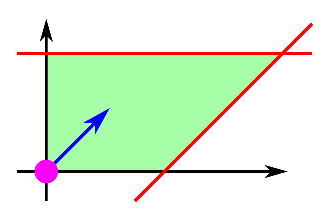
\includegraphics[width=\columnwidth]{images/simplex12.eps}%
\figcaption{Geometrical interpretation of the maximization problem. The constraints are in red, the blue arrow corresponds to the gradient of the objective function, the feasible area is shaded, the purple point is the origin (the point described by the first dictionary).}}

\figurecol{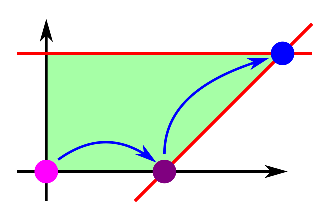
\includegraphics[width=\columnwidth]{images/simplex15.eps}%
\figcaption{The current point after the first pivot is $(2,0)$, and after the second $(4,2)$.}}



\end{multicols}























%Instead of setting the cobasis to zero, lower and/or upper bounds can be kept for each variables, alongside with a valuation (initialized at $0$ for every variable). The original variables don't have bounds. Once again the valuation of the variables of the cobasis is sufficient to determine the valuation of the basis. The dictionary stays identical (only the constants' column becomes useless). Here the variables can be positive or negative.

%The first phase will be to reach the feasible area, i.e. ensure that for all the variables, the valuation respects the bounds. To do so, let's pick a variable $i$ in the basis which bounds are not satisfied, without loss of generality let's assume the upper bound is not satisfied. Then let's pivot it with a cobasic variable $j$ smaller than its upper bound if $a_{ij}>0$ or greater than its lower bound if $a_{ij}<0$. Then the variable $i$ is assigned to its upper bound and the new valuation of the basis is computed. This operation is to be repeated until all the variables are in their bounds, a feasible point is found, or until no suitable pivot can be found, the feasible area is empty.

%The second phase, the optimization is very similar to the classic algorithm, instead of pushing the cobasis to zero, the valuation is fixed and the variables are pushed to their upper or lower bound (depending on the objective) when they are sent in the cobasis. This second phase will not be used in this paper.






\subsection{Fukuda's algorihm}

%vague overview
Fukuda's algorithm allows to enumerate all the vertices of an $\mathcal{H}$-polytope included in the positive orthant ($(\mathbb{R}_+)^d$, all its points have non-negative coordinates) for which the origin is a vertex. This algorithm uses the pivoting scheme of the simplex to explore the polytope. 

It is based on a simple idea: starting from any vertex, the simplex algorithm allows to reach a vertex maximizing a linear function by a unique (thanks to Bland's rule) path among the vertices. The algorithm picks a function maximized only by the origin on the positive orthant and walks backward on all the paths leading to it from all the vertices. Every time a vertex is encountered, it is output.

The first thing to do is to find the end of all these paths: the dictionary corresponding to the origin. It roughly consists in taking the canonical base as cobasis and the set constraints as the basis and setting $-\sum_{i=0}^d x_i$ as the cost function. All the possible pivots are tried from this dictionary. If a pivot leads to a primal feasible dictionary (defining a vertex inside the polytope) for which the Bland's method leads back to the previous point it is said to be a valid reverse Bland's pivot. It means that a step backward has been made on one of the paths, the new point is output, and the method has to be applied from this new point.

However, if a vertex is defined by more hyperplanes than required, several dictionaries will describe the same point, which is said to be degenerated. Fukuda overcomes this problem by defining a partial order on the dictionaries. This order corresponds to a lexicographic order on the basis for the dictionaries defining the same point. A point is only output if its dictionary is lexicographical minimal. Note that the algorithm continues on the dictionary, even if it is not lexicographical minimal.

If the origin is degenerated, then all the optimal dictionaries defining it have to be found. This is done by using a procedure very similar from the one above: by looking only at the hyperplanes redefining the origin, every pivot is tried. The difference is instead of using the Bland's rule, a variation of the dual Bland's rule is used. If the new dictionary is dual feasible (still an optimal for the cost function) and the dual Bland's rule brings it back to the previous one, then the new dictionary is valid with respect to the dual Bland's rule etc. This research presents the same uniqueness properties than the previous one. The previous research has to be launched from every dictionary obtained this way.

The following example illustrates Fukuda's algorithm on a polytope with no degenerated vertex:

\begin{example}
	Let $h$ be the polytope included in the positive orthant and the half-space $x+2y\leq 4$ (plus the positive orthant, i.e. $-x\leq 0$ and $-y\leq 0$) in $\mathbb{R}^2$.\\
	First step, the optimal dictionary:
	\begin{tabular}{| c | c || c || c c |}
	\hline	
	$x$ & $y$ & const & & \\
	$\downarrow$ &$\downarrow$ &$\downarrow$ & & \\
	\hline
	\hline	
   	$-1$ & $-2$ & $4$ & = & $s_1$\\ \hline \hline	
   	$-1$ & $-1$ & $0$ & $\leftarrow$ & obj \\
   	\hline	
 	\end{tabular}, 
 	$(x,s_1)$ and $(y,s_1)$ are both valid reverse Bland's pivot and gives respectively:
 	\begin{tabular}{| c | c || c || c c |}
	\hline	
	$s_1$ & $y$ & const & & \\
	$\downarrow$ &$\downarrow$ &$\downarrow$ & & \\
	\hline
	\hline	
   	$-1$ & $-2$ & $4$ & = & $x$\\ \hline \hline	
   	$1$ & $1$ & $-4$ & $\leftarrow$ & obj \\
   	\hline	
 	\end{tabular}
 	for the point $(4,0)$ and
 	\begin{tabular}{| c | c || c || c c |}
	\hline	
	$x$ & $s_1$ & const & & \\
	$\downarrow$ &$\downarrow$ &$\downarrow$ & & \\
	\hline
	\hline	
   	$-\frac{1}{2}$ & $-\frac{1}{2}$ & $2$ & = & $y$\\ \hline \hline	
   	$-\frac{1}{2}$ & $-\frac{1}{2}$ & $-2$ & $\leftarrow$ & obj \\
   	\hline	
 	\end{tabular}
 	for the point $(0,2)$. These two dictionaries have no valid reverse Bland's pivot, the enumeration is done.
	\label{example-fukuda}
\end{example}

\paragraph{Complexity:} for $n$ half-space in a space of dimension $d$, Fukuda gives a complexity of $O(nd(n+d)g)$, where $g$ is the number of vertices of the polyhedron, counted with their multiplicity (a degenerated vertex can be define in several ways, it is counted several times). 
\section{Contribution}
\subsection{The vertex enumeration for unbounded polyhedra}
\begin{frame}{Changing coordinates}
Requirement: put $0$ in the feasible area and ensure the variables are positive.

\vspace*{0.5cm}

\begin{block}{Finding a vertex}
\begin{itemize}
\item Reach the feasible area (simplex).
\item Pivot the dictionary into obtaining a cobasis constituted only by slack variables.
\item Push the cobasis to its bounds gives a vertex.
\end{itemize}
\end{block}

\end{frame}

\begin{frame}{Detecting the linealty space}

The linealty space is the biggest affine subspace included in the polyhedron.

\vspace*{0.2cm}

\begin{columns}[c]
\begin{column}{5cm}
Example with $-1\leq x+y\leq 1$.\\

\begin{tabular}{| c | c || c c |}
	\hline	
	$x$ & $y$ & & \\
	\hline
	\hline	
   	$-1$ & $-1$ & = & $s_1$\\ \hline	
   	$-1$ & $-1$ & = & $s_2$\\ \hline 
\end{tabular}

\vspace*{0.2cm}

\only<2,3>{\begin{tabular}{| c | c || c c |}
	\hline	
	$s_1$ & $y$ & & \\
	\hline
	\hline	
   	$-1$ & $-1$ & = & $x$\\ \hline	
   	$1$ & $0$ & = & $s_2$\\ \hline 
\end{tabular}

\vspace*{0.2cm}
$(-1,1)$ is a linealty direction.}
\end{column}
\begin{column}{5cm}
\begin{figure}
\only<1,2>{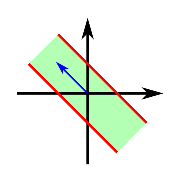
\includegraphics[scale=1.5]{images/linealty.eps}}
\only<3>{
\includegraphics[scale=1.5]{images/linealty2.eps}}
\end{figure}
\end{column}
\end{columns}


\end{frame}

\begin{frame}{Detecting the cone}
Cones' vectors are detected during Fukuda's algorithm.
\begin{block}{Proposition}
For all vertices, any unbounded direction with $d-1$ variables of the cobasis saturated belongs to the cone. The cone equals the conic hull of these vectors.
\end{block}


\vspace*{0.1cm}

\begin{columns}[c]
\begin{column}{5.5cm}
Example with $x-y\leq 1$.\\

\begin{tabular}{| c | c | c || c c |}
	\hline	
	$x$ & $y$ & & & \\
	\hline	
  	$-1$ & $1$ & $1$ & = & $s_1$\\ \hline	
   	$-1$ & $-1$ & & $\rightarrow$ & obj \\ \hline 
\end{tabular}

\vspace*{0.1cm}


\visible<3,4>{\begin{tabular}{| c | c | c || c c |}
	\hline	
	$s_1$ & $y$ & & & \\
	\hline	
  	$-1$ & $1$ & $1$ & = & $x$\\ \hline	
  	$1$ & $-2$ & & $\rightarrow$ & obj \\ \hline 
\end{tabular}}

\visible<4>{\vspace*{0.2cm}
$(0,1)$ and $(1,1)$ are conic directions.}
\end{column}
\begin{column}{5cm}
\only<1>{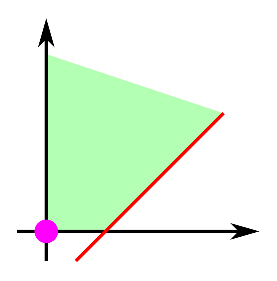
\includegraphics[width=4cm]{images/cone1.eps}}
\only<2>{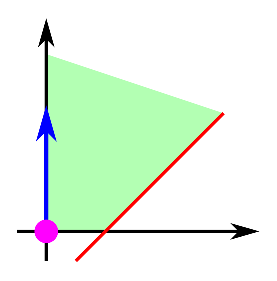
\includegraphics[width=4cm]{images/cone2.eps}}
\only<3>{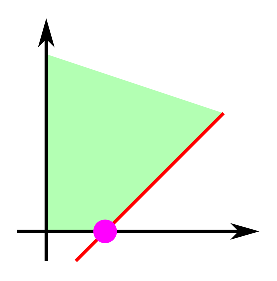
\includegraphics[width=4cm]{images/cone3.eps}}
\only<4>{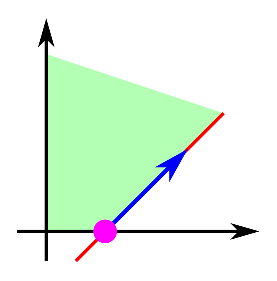
\includegraphics[width=4cm]{images/cone4.eps}}
\end{column}
\end{columns}

\end{frame}

\subsection{The convex hull problem}
\begin{frame}{The convex hull for bounded polyhedra}
In geometry, vertices and half-space are dual notions. The transformation is $a \leftrightarrow a.x \leq 1 $.
\begin{figure}
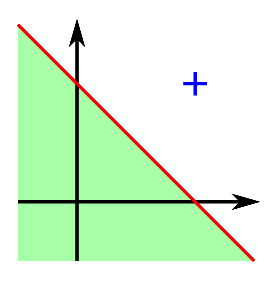
\includegraphics[scale=0.7]{images/dual.eps}

Duality between a vertex $(1,1)$ and an half-space $x+y \leq 1$
\end{figure}

\vspace*{-0.5cm}

\begin{theorem}
Let $P$ be a bounded polyhedron, if $0\in P$ then $P=P^{\Delta\Delta}$.
\end{theorem}

Starting from $P$, finding the vertices of $P^\Delta$ gives the convex hull of $P^{\Delta\Delta}$.
\end{frame}

\begin{frame}{An example of the convex hull algorithm}
\begin{itemize}
\visible<2->{\item Compute $P^\Delta$.}
\visible<3->{\item Enumerate the vertices.}
\visible<4->{\item Compute $P^{\Delta\Delta}$.}
\end{itemize}

\begin{figure}
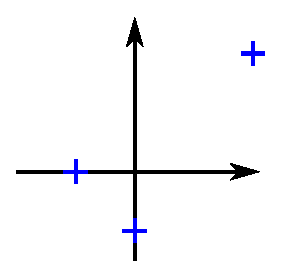
\includegraphics[scale=1]{images/dual11.eps}
\hspace*{0.5cm}
\only<2>{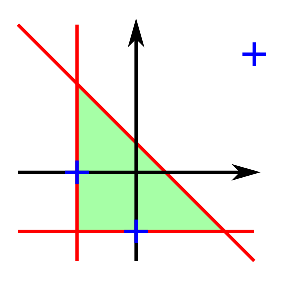
\includegraphics[scale=1]{images/dual2.eps}}
\only<3>{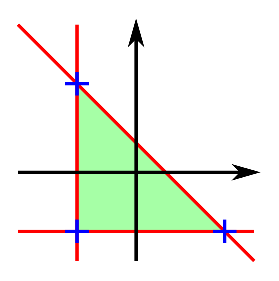
\includegraphics[scale=1]{images/dual3.eps}}
\only<4>{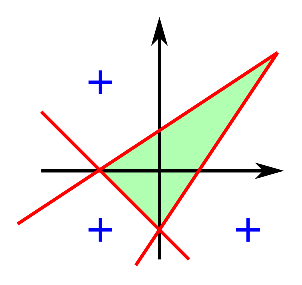
\includegraphics[scale=1]{images/dual4.eps}}
\only<5>{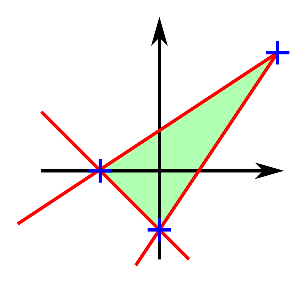
\includegraphics[scale=1]{images/dual5.eps}}

An example in two dimensions.
\end{figure}
\end{frame}

\begin{frame}{Finding the conic hull with the convex hull}
\begin{itemize}
\item consider the vectors as vertices and add the origin;
\item find the convex hull;
\item delete the hyperplanes not including the origin.
\end{itemize}
\begin{figure}
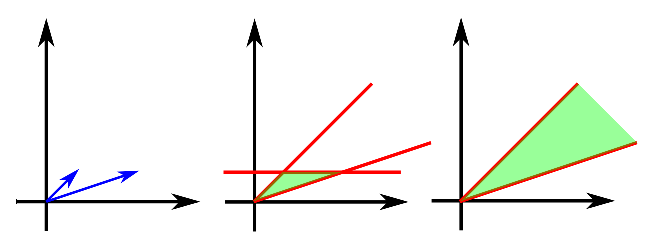
\includegraphics[scale=1]{images/conehull.eps}

An example in two dimensions.
\end{figure}
\end{frame}

\begin{frame}{The convex hull for polyhedron}
Any $V$-polyhedron $P=conv(V)+cone(C)$ can be written as the intersection of a cone and an hyperplane:

$P=Cone\left(
 \begin{pmatrix}
 0 \\
 C 
 \end{pmatrix},
 \begin{pmatrix}
 1 \\
 V 
 \end{pmatrix}\right) \cap \{(1,x)|x\in\mathbb{R}^d\}$
 
 %\vspace*{-0.7cm}
 
\begin{figure}

\includegraphics[scale=1.5]{images/projection.eps}

A $V$-polyhedron as an intersection.
\end{figure}
\end{frame}

\begin{frame}{Complexity result}
Theoretical complexity of Fukuda's algorithm: $nd(n+d)g$. $g\in \left[1;
\begin{pmatrix}
 d\\
 n 
 \end{pmatrix}\right]$

Cost of the algorithms:
\begin{itemize}
\item detect the linealty: cost of the simplex;
\item detect the cone: smaller than Fukuda's algorithm ($nd$ per vertex);
\item switch to the dual: $nd$.
\end{itemize} 

Faster than the current implementation, even in small dimension.

\end{frame}

\section{Conclusion}
\begin{frame}{Complexity result}
\begin{block}{Contribution}
\begin{itemize}
\item Adaptation of Fukuda's algorithm.
\item Implementation.
\end{itemize}
\end{block}

\begin{block}{$\mathcal{H}\rightarrow\mathcal{V}$}
\begin{itemize}
\item Adapt for Fukuda. $\rightarrow$ find linealty space.
\item Fukuda's algorithm find vertices and cone directions.
\end{itemize}
\end{block}


\begin{block}{$\mathcal{V}\rightarrow\mathcal{H}$}
\begin{itemize}
\item Transform into a cone and take the geometric dual.
\item Find the vertices of the dual and take their duals to find the convex hull.
\end{itemize}
\end{block}
\end{frame}

%\begin{frame}{Going further?}

%\end{frame}

%\beginbackup
%\input{annexes.tex}
%\backupend

\end{document}

